% ====================================================================
%+
% SECTION NAME:
%    photoz.tex
%
% CHAPTER:
%    cosmology.tex
%
% ELEVATOR PITCH:
%    Photometric redshifts are an intermediate data product that comprises
%    a key input for many investigations of galaxies and cosmology.  They
%    represent "static science", but we need them to have high quality after
%    the first year and at each "data release" thereafter.
%
% COMMENTS:
%    Updated Wed May 18 by MLG.
%    Minor updates to figures and captions, Sep 14 by MLG.
%
% BUGS:
%
%
% AUTHORS:
%   Melissa Graham, Sam Schmidt, Andy Connolly, Zeljko Ivezic
%-
% ====================================================================
\clearpage
\section{Photometric Redshifts}
\def\secname{photoz}\label{sec:\secname}

\credit{MelissaGraham},
\credit{SamSchmidt},
\credit{connolly},
\credit{ivezic}

\subsection{Introduction}

Photometric redshifts are an essential part of
every cosmology probe within LSST.  The principal concern for LSST
photo-$z$ performance is to meet the stringent requirements on redshift
uncertainty, bias, and catastrophic outlier rate as laid out in the
Science Requirements document. Photo-$z$'s are dependent on precise
measurements of galaxy colors, thus cadence and depth variations must be
examined as a function of all six LSST filter bandpasses.  Overall image
depth and signal-to-noise is our primary concern. For studies of Large
Scale Structure, Weak Lensing, Clusters, and Supernova host galaxies,
survey uniformity is desired for the full depth survey, while the
temporal details of how we reach full depth are not as important as
uniformity both as a function of sky position and observing conditions.
However, as we desire science-grade photometric redshifts after one year
of operations, two years, and so forth, the cadence must meet some basic
requirements for the six-band system at least on the timescales of the
yearly data releases.


\textbf{Specifications.} The Science Requirements Document (SRD; \citealt{LPM-17}) defines
the minimum statistical specifications for photometric redshifts for an
$i<25$, magnitude-limited sample of $4\times10^9$ galaxies from
$0.3<z<3.0$ as: (1) the root-mean-square of the error in photo-$z$
must be $\sigma < 0.02$; (2) the fraction of outliers must be $<10\%$;
and (3) the average bias must be $<0.003$.
The details for how these statistics are calculated are discussed in the Metrics section below.
With this in mind, we are developing software to show that our photo-$z$ algorithms
can meet specifications for LSST baseline parameters and to simulate the
impact of deviations from the 10-year baseline plan on photo-$z$
statistics.

\textbf{Planned Experiments.} This software is designed to allow the
user to modify LSST baseline parameters, simulate a set of test galaxy
observations (i.e., magnitudes with errors appropriate for the given
LSST parameters) from a training catalog with ``true" magnitudes and
redshifts and a realistic intrinsic dispersion in color, magnitude, and
redshift, run a photometric redshift algorithm on the test galaxies
(i.e., matching in color-space to the training catalog), and output
statistics for analysis. Modifiable LSST input parameters will include:
the limiting magnitude applied to the galaxy catalogs (e.g., $i<25$);
the number of visits per filter; the number of years of LSST
observations that have passed (this can be a fraction of a year);
systematic offsets to the magnitudes in each filter (default $=0$); and
coefficients for the magnitude uncertainties in each filter (default
$=1$).  Output for user analysis will include catalogs of $z_{\rm phot}$
and the metrics for photo-$z$
in any desired redshift range. For example, we will be able to vary the
total number of $u$-band visits and examine how this affects the
fraction of outliers at 1, 5, and 10-years of the survey. In this
software, parameters of the photo-$z$ algorithm itself will also be
modifiable, allowing us to test options in the algorithms against
various LSST observing strategies.

\textbf{Currently implemented photo-$z$ algorithm.} We draw $N_{\rm
test}$ ``test" and $N_{\rm train}$ ``training" galaxies from a catalog of
simulated galaxies (ensuring no overlap), determine their
magnitude uncertainties as appropriate for the LSST parameters, randomly
scatter their magnitudes to induce an observational error, and calculate
the associated colors and color errors. We calculate the Mahalanobis
distance \citep{Mahalanobis1936} in color space between each test galaxy and all training
catalog galaxies, and identify a color-matched subset using a threshold
defined by the $\chi^2$ percentage point function at 68\%. We draw a
random color-matched training galaxy and use its redshift as the
photo-$z$ for that test galaxy. We then calculate our statistical
metrics on the photometric redshifts for the test sample, using each
test galaxy's original catalog redshift as the ``true'' redshift. This
process is open to substituting alternate photometric redshift
algorithms, a variety of galaxy catalogs, and/or adding priors based on
e.g., apparent magnitude. For this experiment, we always assume that the
training set galaxies have photometric errors equivalent to that of the
full-depth (i.e., 10-year) LSST catalog.

\subsection{Metrics}

The primary metrics we will use to evaluate LSST
observing strategies with respect to the SRD photo-z specifications are the
robust standard deviation, the robus bias, and the fraction of outliers. For all test
galaxies we calculate $\Delta z = (z_{\rm true} - z_{\rm phot}) /
(1+z_{\rm true})$, and identify galaxies in the interquartile range (IQR) of $\Delta z$.
The robust standard deviation is calculated by dividing the full-width of the IQR by 1.349 (i.e., assuming a Gaussian distribution, which we find to be appropriate).
The robust bias is the mean value of $\Delta z$ for IQR galaxies.
Outlier galaxies are identified as those with $\Delta z$ exceeding the larger of 0.06 or 3$\sigma$, 
where $\sigma$ is the robust standard deviation for all galaxies with $0.3 \leq z_{\rm phot} \leq 3.0$.
The IQR is used to exclude outliers from influencing these statistics; in other words, the robust
standard deviation and bias are for a subset of ``good" photo-$z$'s.

\subsection{Initial Results}

To demonstrate this software with a
preliminary analysis, we apply the currently implemented photo-$z$
algorithm to a galaxy catalog based on the Millennium simulation \citep{2005Natur.435..629S},
which uses the galaxy formation models of \citep{2014MNRAS.439..264G}
and was constructed using the lightcone techniques described by \cite{2013MNRAS.429..556M}.
We first cull the catalog to galaxies with $i$-band magnitude $<25.05$
(the condition of $i<25$ is applied after scattering based on their magnitude errors),
and then randomly draw training and test galaxy samples (with at least a 4$\times$ more
galaxies in the training sample than the test sample). For this
demonstration we show how the photo-$z$ metrics evolve with respect to
two of the basic LSST parameters: the year of the survey, and the number
of $u$-band visits. When we simulate results in a given year of LSST, we
assume uniform progression in all filters (i.e., the total number of
visits per filter, \texttt{[56, 80, 184, 184, 160, 160]} in
\texttt{[u,g,r,i,z,y]}, is distributed evenly over all years). When we
simulate the LSST 10-year results for a given number of $u$-band visits,
the visits removed/added to $u$-band are added/subtracted evenly to/from
the other five filters. The results of these tests are presented in
Figure~\ref{fig:redshifts} and~\ref{fig:metrics}. For example, in this
demonstration we can see that the $u$-band is necessary to limit scatter
at $z<0.5$ and $z>2.0$.

\begin{figure}[h]
\begin{center}
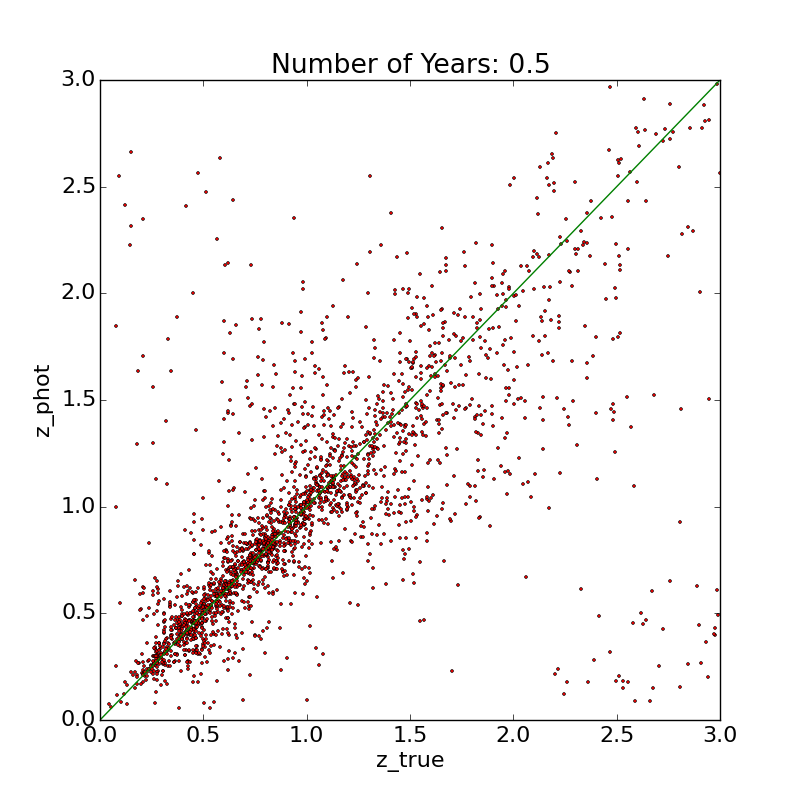
\includegraphics[width=5cm]{figs/photoz/nyears_cat05.png}
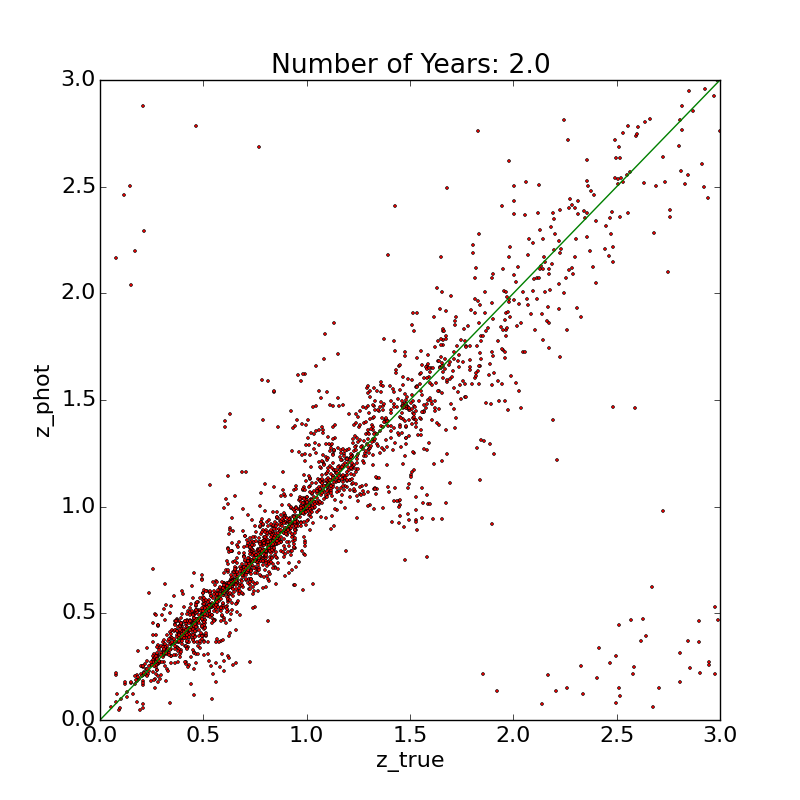
\includegraphics[width=5cm]{figs/photoz/nyears_cat20.png}
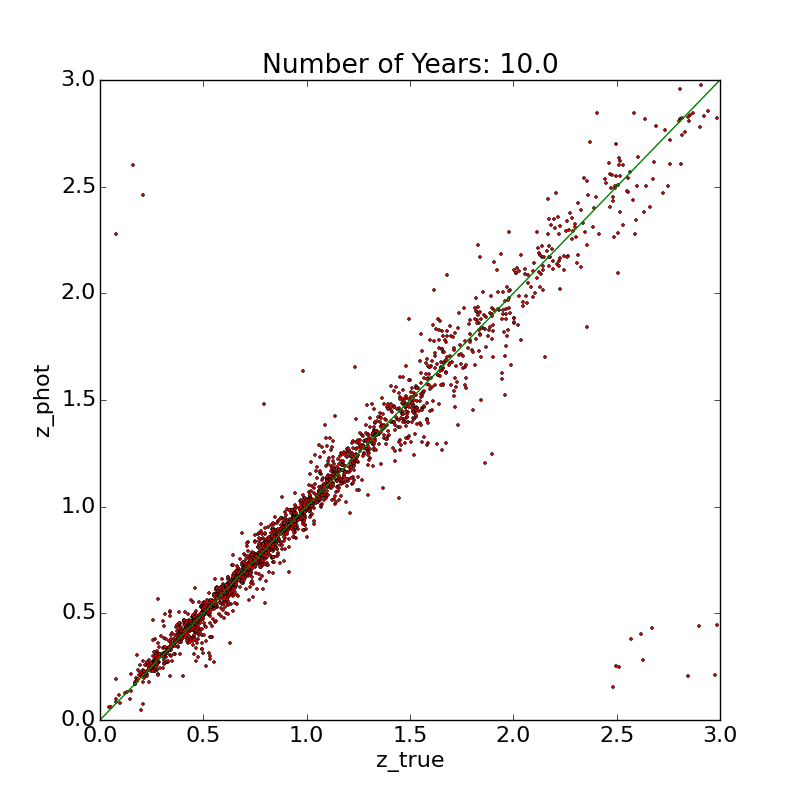
\includegraphics[width=5cm]{figs/photoz/nyears_cat100.png}
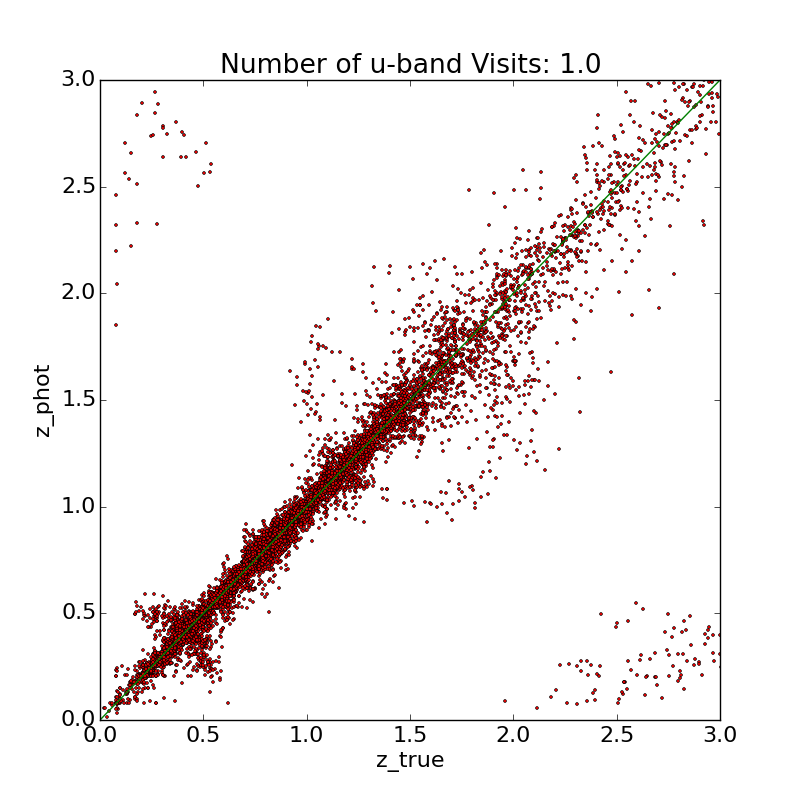
\includegraphics[width=5cm]{figs/photoz/uvisits_cat1.png}
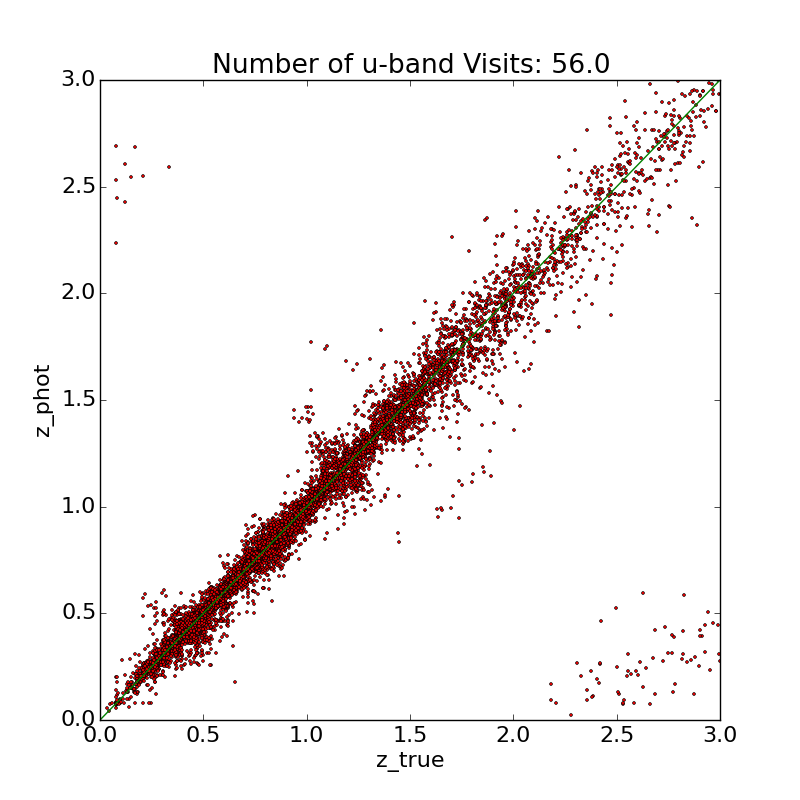
\includegraphics[width=5cm]{figs/photoz/uvisits_cat4.png}
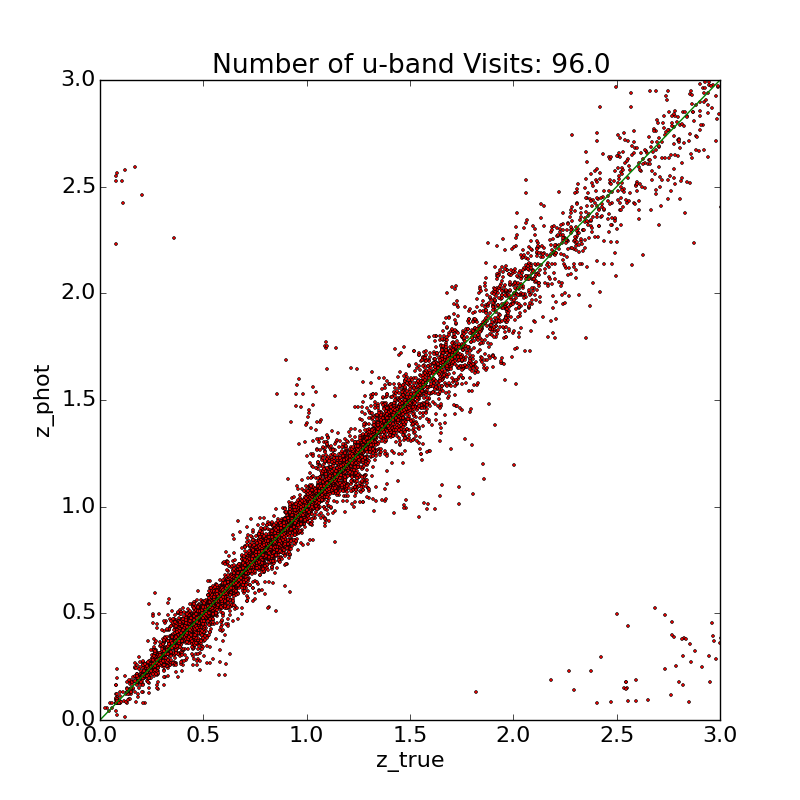
\includegraphics[width=5cm]{figs/photoz/uvisits_cat6.png}
\caption{Photometric vs. spectroscopic (i.e., catalog truth) redshifts
for our preliminary simulations. Across the top row we show results from
0.5, 2.0 and 10.0 years of the LSST survey using catalogs with 50000 test
and 1000000 training galaxies. Overall, the photo-$z$'s clearly improve with time
as the survey progresses. Across the bottom row we show results for $0$,
$56$ (baseline), and $96$ $u$-band visits, using the same test and training
galaxies. Between the left-most and middle plot of
the bottom row, representing 0 and 56 (baseline) $u$-band visits
respectively, we see that $u$-band data is necessary to limit scatter in
the photo-$z$'s, especially at $z<0.5$ and $z>2.0$.
\label{fig:redshifts}}
\end{center}
\end{figure}

\begin{figure}[h]
\begin{center}
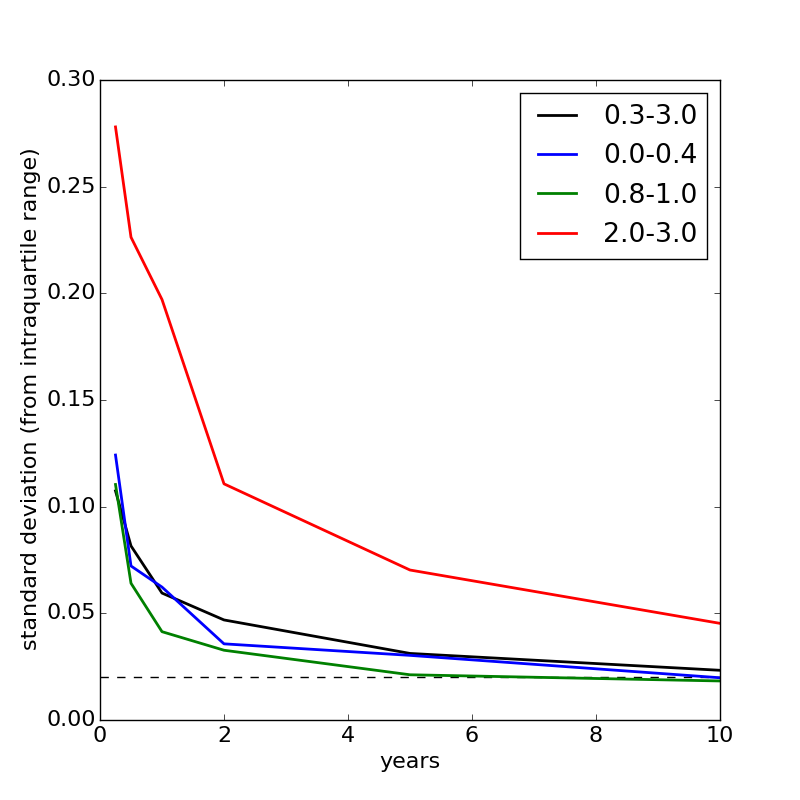
\includegraphics[width=5cm]{figs/photoz/nyears_IQR.png}
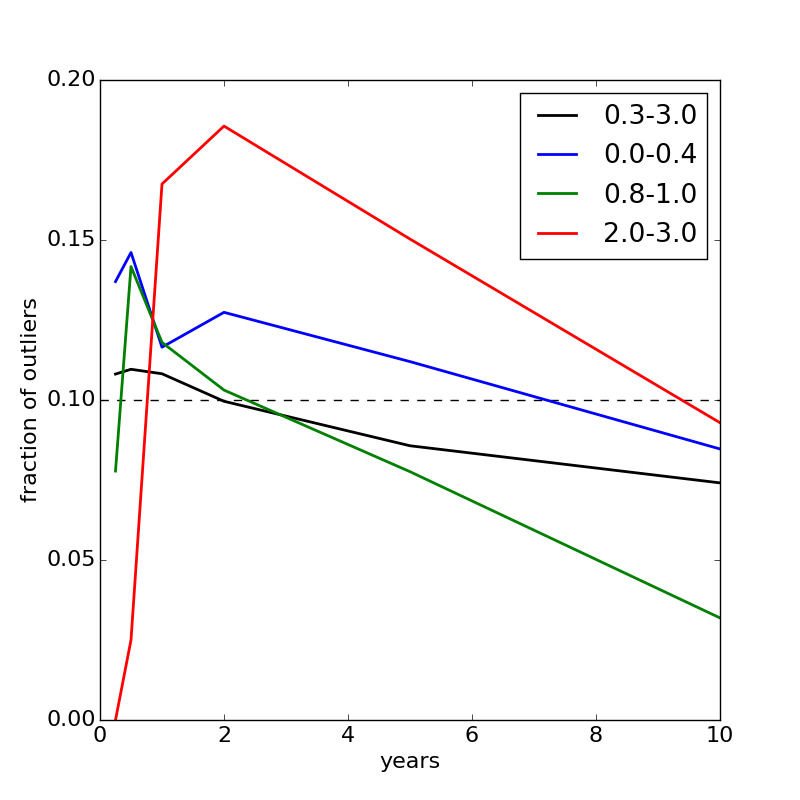
\includegraphics[width=5cm]{figs/photoz/nyears_fout.png}
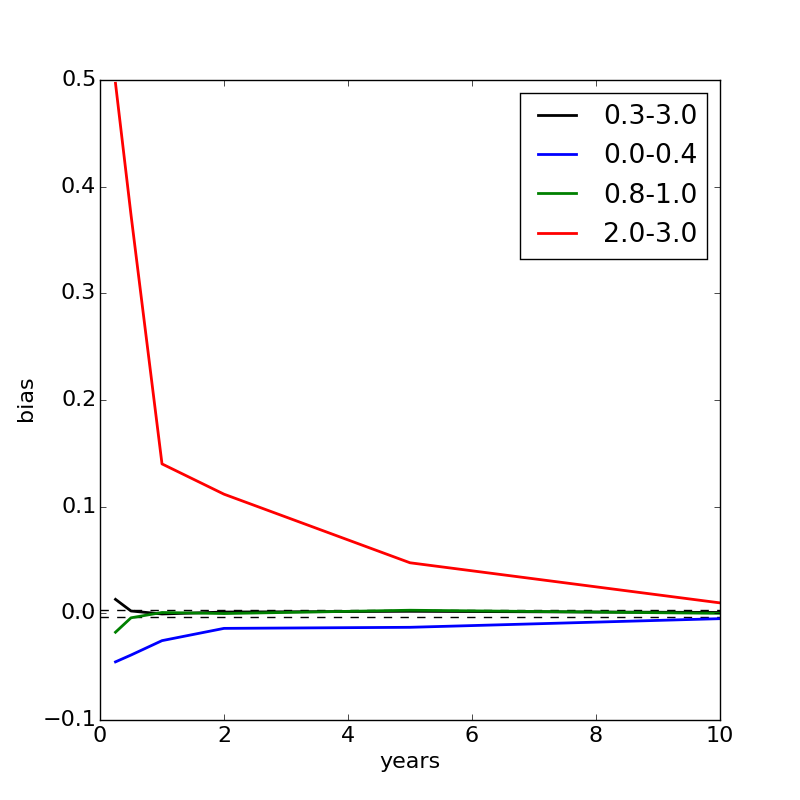
\includegraphics[width=5cm]{figs/photoz/nyears_bias.png}
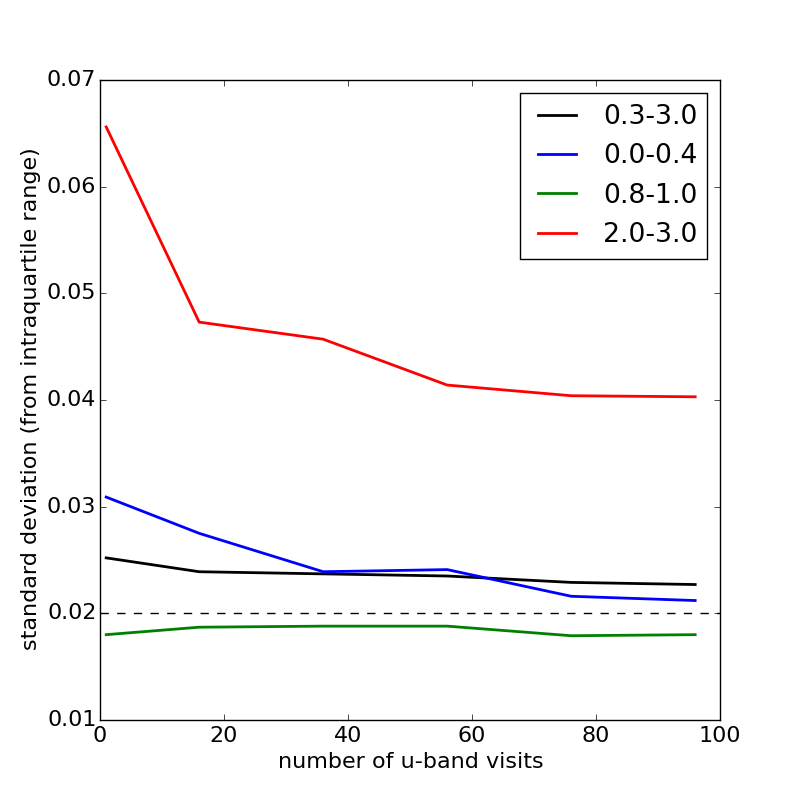
\includegraphics[width=5cm]{figs/photoz/uvisits_IQR.png}
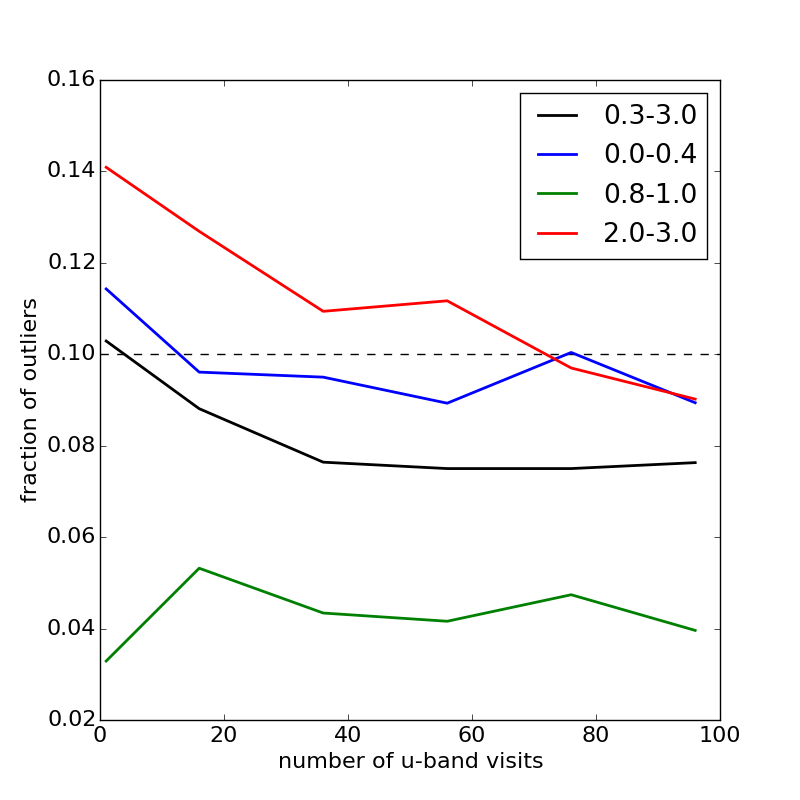
\includegraphics[width=5cm]{figs/photoz/uvisits_fout.png}
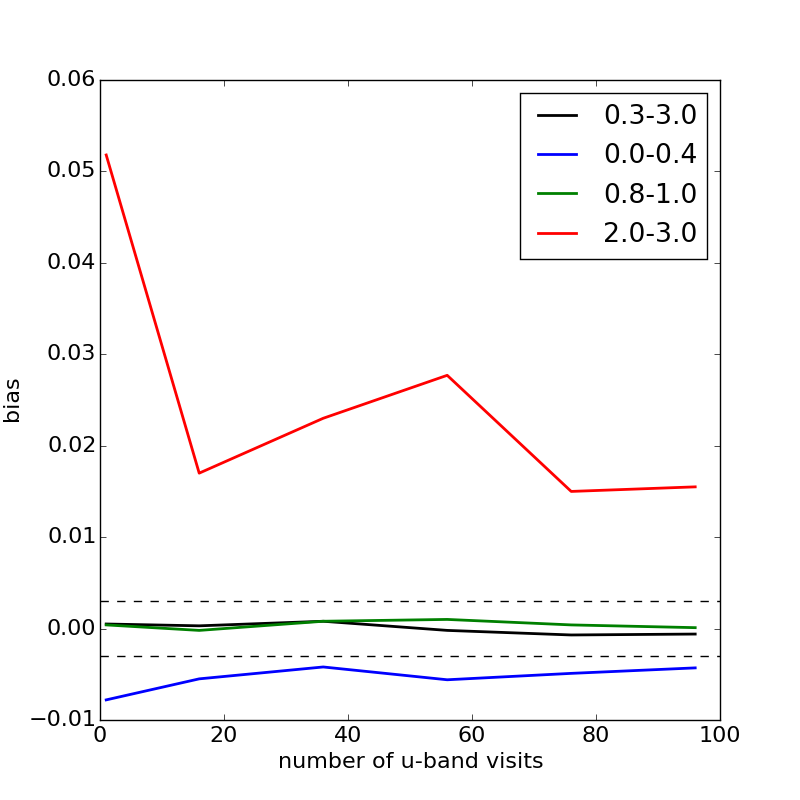
\includegraphics[width=5cm]{figs/photoz/uvisits_bias.png}
\caption{Three photo-$z$ metrics as a function of LSST parameters. From
left to right, the y-axis is the robust standard deviation, the fraction of
outliers, and the robus bias. The top row shows these statistics as a function
of the number of years of LSST survey, and the bottom row shows them as
a function of the number of $u$-band visits. Colors show these relations
for four bins in redshift: 0.3--3.0 (black), 0.3--0.5 (blue), 0.9--1.1
(green), and 2.0--3.0 (red). Grey lines mark the SRD specification for
each statistical measure. The fraction of outliers in the low-$z$ bin of 0.3--0.5
actually increases with time because the standard deviation decreases, as can
also be seen in the top panels of Figure \ref{fig:redshifts}.
\label{fig:metrics}}
\end{center}
\end{figure}


\subsection{Discussion}

\textbf{Additional considerations for observing strategy.} As mentioned
above, overall image depth and signal-to-noise is our primary concern,
so we are not testing changes in e.g., the inter-night gap time or the
exposure time of individual visits.  Our software is instead focused on
modifying other LSST parameters such as systematic offsets to the
magnitudes in each filter and/or coefficients for the magnitude
uncertainties in each filter in order to simulate improvements or
degradations the system throughput, sky background brightness, and other
such factors. We also aim to test airmass distributions (i.e., changes
to the effective filter functions), different progression rates for
filters (e.g., a scenario in which we complete all $u$-band by year 2),
scenarios in which some areas of sky have better/worse coverage at any
given time, and so forth. In all respects we are open to suggestions
from the community.

\textbf{Considerations for building the real training catalog.} All
photometric redshift algorithms require training set data consisting of
objects with secure spectroscopic redshifts.  For LSST, many of these
will be contained in a small number of training/calibration fields (e.g.
COSMOS, VVDS).  Imaging these fields to full depth in all six bands
early in the survey (but under the range of observing conditions
expected for the ten year survey) will be key to characterizing
performance.  Inclusion of these patches of full-depth imaging must be
included in any cadence design. Future simulations of photo-$z$ results
can include varying the quality of the training catalog obtained by
LSST.

\textbf{Integration with MAF.} One way to extend our program to be able
to evaluate observing strategies simulated with \OpSim could be to use
the MAF to enable us to simulate representative samples of galaxies
across the mock LSST sky, and compute the metrics we have defined.
It may be possible to avoid such a large computation by first defining
some intermediate diagnostic metrics, such as the $u$-band coverage, and
working out how our higher level metrics depend on them, using some
approximate interpolation formulae.

\textbf{Connecting to the Dark Energy Figure of Merit.} The metrics we
have defined here should be able to be related to the DETF Figure of
Merit, but because photo-zs affect all of the LSS, WL and CL
cosmological probes, this step may need to wait until a joint
Figure of Merit MAF metric is developed.

% --------------------------------------------------------------------
%
 \subsection{Conclusions}

 Here we answer the ten questions posed in
 \autoref{sec:intro:evaluation:caseConclusions}:

 \begin{description}

 \item[Q1:] {\it Does the science case place any constraints on the
 tradeoff between the sky coverage and coadded depth? For example, should
 the sky coverage be maximized (to $\sim$30,000 deg$^2$, as e.g., in
 Pan-STARRS) or the number of detected galaxies (the current baseline but
 with 18,000 deg$^2$)?}

 \item[A1:] Since increasing the areal coverage comes at the expense of depth per pointing, this will adversely affect the photometric redshift quality. We estimate that only ~80\% of the galaxies would then meet the signal-to-noise threshold for photo-z analysis, but that this would be more than offset by the extra area and the final catalog would be ~108\% the size. Although this appears to be a net gain, it would change the redshift range for analysis.

 \item[Q2:] {\it Does the science case place any constraints on the
 tradeoff between uniformity of sampling and frequency of  sampling? For
 example, a rolling cadence can provide enhanced sample rates over a part
 of the survey or the entire survey for a designated time at the cost of
 reduced sample rate the rest of the time (while maintaining the nominal
 total visit counts).}

 \item[A2:] The sampling frequency is not important to photo-z, but building a uniform depth as a function of time would enable early science that relies on photo-z, so long as this depth is distributed across all filters. This distribution probably does not need to be exactly even, but tolerances have yet to be studied (e.g. rolling cadence may lead to seasonal variations that induce large-scale patchiness in the depth). However, sampling to full depth in all of the bands except g would have a negative impact, for example.

 \item[Q3:] {\it Does the science case place any constraints on the
 tradeoff between the single-visit depth and the number of visits
 (especially in the $u$-band where longer exposures would minimize the
 impact of the readout noise)?}

 \item[A3:] Photo-z would be improved if the u-band magnitude uncertainties could be further minimized, so long as this does not take away visits from other filters. If this could be done by longer u-band exposures during single-visits but less overall u-band visits, that would be good for photo-z.

 \item[Q4:] {\it Does the science case place any constraints on the
 Galactic plane coverage (spatial coverage, temporal sampling, visits per
 band)?}

 \item[A4:] Galactic plane coverage is not applicable to photo-z.

 \item[Q5:] {\it Does the science case place any constraints on the
 fraction of observing time allocated to each band?}

 \item[A5:] We find that at least ~20 u-band visits are necessary for the photo-z statistics to meet specifications.

 \item[Q6:] {\it Does the science case place any constraints on the
 cadence for deep drilling fields?}

 \item[A6:] Cadence of the DDF is not applicable to photo-z.

 \item[Q7:] {\it Assuming two visits per night, would the science case
 benefit if they are obtained in the same band or not?}

 \item[A7:] Intra-night filter changes do not affect photo-z.

 \item[Q8:] {\it Will the case science benefit from a special cadence
 prescription during commissioning or early in the survey, such as:
 acquiring a full 10-year count of visits for a small area (either in all
 the bands or in a  selected set); a greatly enhanced cadence for a small
 area?}

 \item[A8:] Photometric redshift analysis would be greatly assisted by acquiring a full 10-yr count of visits in all six bands for a small area during commissioning or early in the survey, especially if these assets are in regions covered by existing spectroscopic surveys.

 \item[Q9:] {\it Does the science case place any constraints on the
 sampling of observing conditions (e.g., seeing, dark sky, airmass),
 possibly as a function of band, etc.?}

 \item[A9:] Preliminary analysis shows that photometric redshifts may benefit by sampling in airmass, especially in the u-band, but a full assessment of the tradeoffs is pending. In general, a more uniform distribution of conditions is a guard against systematics.

 \item[Q10:] {\it Does the case have science drivers that would require
 real-time exposure time optimization to obtain nearly constant
 single-visit limiting depth?}

 \item[A10:] No

 \end{description}


\navigationbar

% ====================================================================
